\documentclass[t]{beamer}
\usepackage{textcomp}
\usepackage{caption}
\usepackage{listings}
\usepackage{amssymb}
\usepackage{minted}

\usetheme{default}
\usebackgroundtemplate{
\includegraphics[width=\paperwidth]{../cpeb_bkground_topleft.pdf}}

\setbeamertemplate{frametitle}{
  \centering\vspace{1mm}\insertframetitle\par\vspace{3mm}
}

\title{\texttt{AXE}}
\subtitle{The Rapid and Accurate Demultiplexer}
\author{Kevin Murray\\\tiny{\texttt{@kdmurray91}\\kevin@kdmurray.id.au}}
\institute{Borevitz Lab, ANU}
\date{\today}

\begin{document}

{
\usebackgroundtemplate{
\includegraphics[width=\paperwidth]{../cpeb_bkground_centered.pdf}}
\begin{frame}
  \titlepage
  \vfill
\end{frame}
}


\begin{frame}{About Me}
  \begin{columns}[b]
    \column{0.6\textwidth}
    \begin{itemize}
      \item Bioinformatician @ Borevitz Lab
      \begin{itemize}
        \item TraitCapture Project Developer
        \item Genomics (Low level Sequence Analysis)
        \item Phenomics (Image analysis)
        \item Sample tracking, data standards, HPC
      \end{itemize}
      \item Starting PhD in Bioinformatics next year
    \end{itemize}
    \column{0.4\textwidth}
    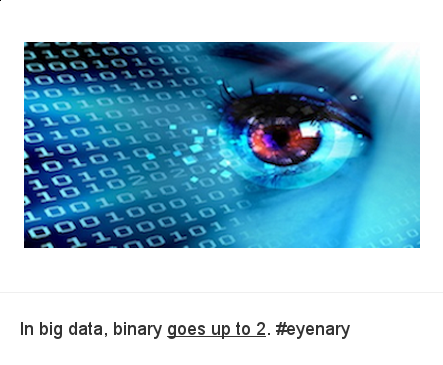
\includegraphics[width=0.8\textwidth]{img/bigdata.png}
  \end{columns}
\end{frame}


\begin{frame}{The High Throughput Problem}
  \begin{columns}[b]
    \column{0.6\textwidth}
    \begin{itemize}
      \item Sequencing $==$  firehose of data
      \item Need to put $>$ 1 sample / lane
      \item Give BRF only one tube
      \item $\therefore$ we need multiplexing
      \item $\therefore$ de-multiplexing
    \end{itemize}
    \column{0.4\textwidth}
    \includegraphics<1|only@1>[width=\textwidth]{img/hiseq.png}
    \includegraphics<2|only@2>[width=0.8\textwidth]{img/firehose.jpg}
  \end{columns}
\end{frame}


\begin{frame}{DNA/Molecular Barcoding}
  \begin{columns}[b]
    \column{0.5\textwidth}
    \begin{itemize}
      \item DNA fragment contains per-sample unique seq.
      \item Sequenced, and ``attached'' to a read
    \end{itemize}
    \column{0.5\textwidth}
    \begin{itemize}
      \item Must be balanced \& staggered
      \item Hamming distance $>$2
    \end{itemize}
  \end{columns}
  \begin{center}
    \includegraphics<1|only@1>[width=0.8\textwidth]{img/simple_barcodes.png}
  \end{center}
\end{frame}

\begin{frame}{So you need a demulitplexer?}
  \begin{columns}[b]
    \column{0.5\textwidth}
    \begin{itemize}
      \item Some studies use kit protocols
      \item Most kits use index reads
      \item Illumina pipeline automatically demuxes these
    \end{itemize}
    \column{0.5\textwidth}
    \begin{itemize}
      \item<2> Many advanced/homebrew protocols use ``in-read''
      \item<2> Must be demultiplexed by user
    \end{itemize}
  \end{columns}
    \begin{center}
      \includegraphics<1|only@1>[width=0.8\textwidth]{img/2ndread_barcodes.png}
      \includegraphics<2>[width=0.8\textwidth]{img/simple_barcodes.png}
    \end{center}
\end{frame}

\begin{frame}{De-multiplex with \texttt{AXE}}
  \begin{columns}[b]
    \column{0.6\textwidth}
    \begin{itemize}
      \item Barcoding scheme requires advanced de-multiplexing
      \item Trie-based lookup algorithm
      \item Fast (PE lane in 5-10 mins)
      \item Implemented in C
      \item CLI and \texttt{libaxe.so} + \texttt{axe.h}
      \item GNU GPL v3+
    \end{itemize}
    \column{0.4\textwidth}
    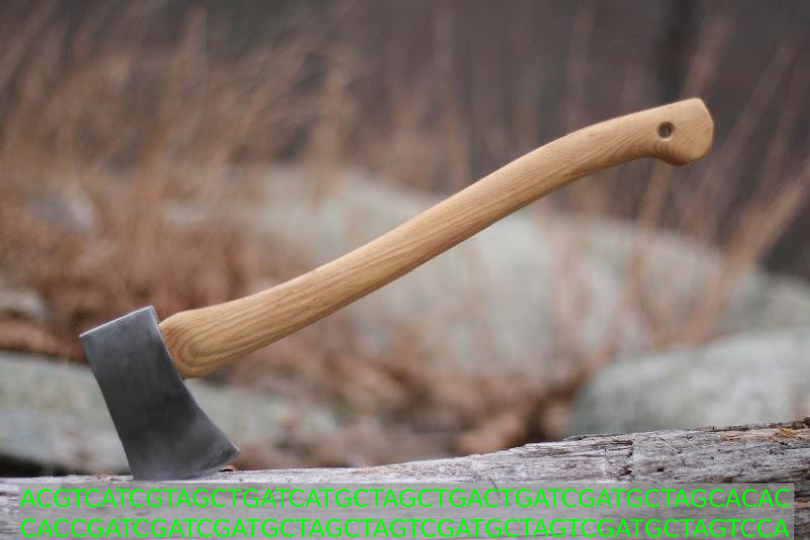
\includegraphics[width=\textwidth]{img/axe.png}
  \end{columns}
\end{frame}

\begin{frame}{Hamming distance}
  \begin{minipage}{\textwidth}
  \begin{itemize}
    \item<1-> {Distance between two strings of equal length \\
       \texttt{ACTGTG} \\
       \texttt{  x x } $= 2$\\
       \texttt{ACAGCG}}
     \item<2|only@2> {Is a poor measure of seq. divergence:\\
       \texttt{ACTGTG} \\
       \texttt{xxxxxx} $= 6$ \\
       \texttt{CTGTGA}}
     \item<3-> {Is a poor measure of seq. divergence:\\
       \texttt{ACTGTG} \\
       \texttt{x.....} $= 1$ \\
       \texttt{-CTGTG}}
     \item<4-> \mint{python}|sum([0 if s1[i] == s2[i] else 1 for i in range(l)])|
     \item<5-> {Good Enough\texttrademark}
  \end{itemize}
  \end{minipage}
\end{frame}

\begin{frame}{A Forest of Tries?}
  \begin{columns}[b]
    \column{0.6\textwidth}
    \begin{itemize}
      \item<1-> Trie is k-ary tree for k letter alphabet
      \item<2-> Lookups are $\mathcal{O}(l)$
      \item<3-> i.e., $\mathcal{O}(1)$ WRT number of items, \textit{a la}
                hash-tables
      \item<4-> Memory efficient (prefixes collapsed)
      \item<5-> Prefix lookups very fast
    \end{itemize}
    \column{0.4\textwidth}
    \includegraphics<1->[width=\textwidth]{img/trie.png}
  \end{columns}
\end{frame}

\begin{frame}{Hamming Mismatch Trie}
  \begin{columns}[b]
    \column{0.6\textwidth}
    \begin{itemize}
      \item Pre-calculate all strings with Hamming dist $d$ from search
      \item Make trie, do lookups
      \item Essentially a FSM
    \end{itemize}
    \column{0.4\textwidth}
    \begin{center}
      \includegraphics<1|only@1>[height=3cm]{img/hamming_precalc.png}
      \includegraphics<2->[height=3cm]{img/hamming_trie.png}
    \end{center}
  \end{columns}
\end{frame}

\begin{frame}{The Algorithm}
  \begin{columns}[b]
    \column{0.6\textwidth}
    \begin{itemize}
      \item Take read
      \item Walk trie w/ start of read
      \item Mark full-length matches
      \item Take longest match
    \end{itemize}
    \column{0.4\textwidth}
    \begin{center}
      \includegraphics<1|only@1>[height=3.6cm]{img/algo-1.png}
      \includegraphics<2|only@2>[height=3.6cm]{img/algo-2.png}
      \includegraphics<3|only@3>[height=3.6cm]{img/algo-3.png}
      \includegraphics<4|only@4>[height=3.6cm]{img/algo-4.png}
      \includegraphics<5|only@5>[height=3.6cm]{img/algo-5.png}
      \includegraphics<6|only@6>[height=3.6cm]{img/algo-6.png}
      \includegraphics<7|only@7>[height=3.6cm]{img/algo-7.png}
      \includegraphics<8|only@8>[height=3.6cm]{img/algo-8.png}
      \includegraphics<9|only@9>[height=3.6cm]{img/algo-9.png}
      \includegraphics<10|only@10>[height=3.6cm]{img/algo-10.png}
      \includegraphics<11|only@11>[height=3.6cm]{img/algo-11.png}
      \includegraphics<12|only@12>[height=3.6cm]{img/algo-12.png}
      \includegraphics<13|only@13>[height=3.6cm]{img/algo-13.png}
    \end{center}
  \end{columns}
\end{frame}

\begin{frame}{I THINK\ldots}
  \begin{itemize}
    \item WARNING: everything I say from here may well be bullshit
    \item These statements are thought through, but please, tell me if I'm
      wrong
    \pause
    \item Ok, time for an IPython Notebook
  \end{itemize}
\end{frame}



\begin{frame}{Thanks}
  \begin{itemize}
    \item Justin Borevitz
    \item Sylvain For\^{e}t
    \item Aaron Chuah
    \item Cam Jack
    \item Jared Streich \& Collin Ahrens ($\beta$-testers)
  \end{itemize}
  \begin{center}
    
\includegraphics[width=0.6\textwidth]{img/spaninq.jpg}
  \end{center}
\end{frame}

\end{document}
